\begin{Example}[wlfpart]{Women's labor-force participation}
To illustrate, \citet{Fox:84,Fox:97} presented survey data on women's labor-force
participation in Canada in 1977.  Women were classified as not working
outside the home (n=155), working part-time (n=42)  or working
full-time (n=66).  Predictor variables were presence/absence of
children, and husband's income; a third variable, region of Canada,
is not considered here.  For these data, it makes sense to model the
log odds for two nested dichotomies:

\begin{itemize*}
\item Working vs. NotWorking
\item Working fulltime vs working parttime.
\end{itemize*}

The data are read in as shown below.
See \datref{dat:wlfdata} for the complete \Dset.  The 3-level variable
\pname{labor} is used to define two dichotomous variables, \pname{working}, and \pname{fulltime}.  Note that \pname{fulltime} is defined
(has non-missing values) only for working women.

\begin{listing}
proc format;
   value labor    /* labor-force participation */
      1 ='working full-time'  2 ='working part-time'
      3 ='not working';
   value kids     /* presence of children in the household */
      0 ='Children absent'  1 ='Children present';
data wlfpart;
   input case labor husinc children region;
   working = labor < 3;
   if working then
      fulltime = (labor = 1);
datalines;
  1  3  15  1  3
  2  3  13  1  3
  3  3  45  1  3
  4  3  23  1  3
  5  3  19  1  3
  {\it ... more data lines ...}
\end{listing}

An initial analysis attempts to fit the proportional odds model, with
the 3-level \pname{labor} variable as the response:

\begin{listing}
proc logistic data=wlfpart nosimple;
   {\bf model labor  = husinc children ;}
   title2 'Proportional Odds Model for Fulltime/Parttime/NotWorking';
\end{listing}

However, the proportional odds assumption is rejected by the score
test (see \outref{out:wlfpart.1}).

\begin{Output}[htb]
\caption{Test of the proportional odds assumption}\label{out:wlfpart.1}
\small
\begin{output}
          Score Test for the Proportional Odds Assumption

             Chi-Square = 18.5641 with 2 DF (p=0.0001)
\end{output}
\end{Output}

Hence, we fit models for each of the \pname{working} and \pname{fulltime}
dichotomies.  The \opt{descending}{LOGISTIC} is used so that in each
case the probability of a 1 response (working, or fulltime) will be
the event modeled.

\begin{listing}
proc logistic data=wlfpart nosimple descending;
   {\bf model working = husinc children ;}
   output out=resultw p=predict xbeta=logit;
   title2 'Nested Dichotomies';
run;
proc logistic data=wlfpart nosimple descending;
   {\bf model fulltime = husinc children ;}
   output out=resultf p=predict xbeta=logit;
\end{listing}

The \stmt{output}{LOGISTIC}s  create the \Dsets\ \pname{resultw} and
\pname{resultf} for plotting the predicted probabilities and logits.
The printed output for the working dichotomy is shown (partially)
in \outref{out:wlfpart.2}.

\begin{Output}[htb]
\caption{Women's labor-force data, analysis of the working/not working dichotomy}\label{out:wlfpart.2}
\small
\begin{output}
                               Response Profile
                          Ordered
                            Value  WORKING     Count

                                1        1       108
                                2        0       155

                  Testing Global Null Hypothesis: BETA=0
                            Intercept
               Intercept       and
   Criterion     Only      Covariates    Chi-Square for Covariates

   AIC           358.151      325.733      .
   SC            361.723      336.449      .
   -2 LOG L      356.151      319.733    36.418 with 2 DF (p=0.0001)
   Score            .            .       35.713 with 2 DF (p=0.0001)

                    Analysis of Maximum Likelihood Estimates

               Parameter Standard    Wald       Pr >    Standardized    Odds
   Variable DF  Estimate   Error  Chi-Square Chi-Square   Estimate     Ratio

   INTERCPT 1     1.3358   0.3838    12.1165     0.0005            .    .
   HUSINC   1    -0.0423   0.0198     4.5751     0.0324    -0.168541   0.959
   CHILDREN 1    -1.5756   0.2923    29.0651     0.0001    -0.398992   0.207
\end{output}
\end{Output}

To interpret the parameter estimates, note that the odds ratio of 0.959
for husband's income
means a 4\% decrease in the odds of working with each \$1000 increase in husband's income; an additional \$10,000 means a decrease in the odds
of working by
\(e^{-.423} = .655\).  Similarly, the effect of having children  corresponds
to an odds of working of .207 compared to those without children.

The output for the fulltime vs. parttime dichotomy is shown in
\outref{out:wlfpart.3}.
Note that nonworking women are excluded in this analysis.

\begin{Output}[htb]
\caption{Women's labor-force data, analysis of the fulltime/parttime dichotomy}\label{out:wlfpart.3}
\small
\begin{output}
                                Response Profile
                          Ordered
                            Value  FULLTIME     Count

                                1         1        66
                                2         0        42

   WARNING: 155 observation(s) were deleted due to missing values for
           the response or explanatory variables.

                   Testing Global Null Hypothesis: BETA=0
                             Intercept
                Intercept       and
   Criterion      Only      Covariates   Chi-Square for Covariates

   AIC            146.342      110.495      .
   SC             149.024      118.541      .
   -2 LOG L       144.342      104.495    39.847 with 2 DF (p=0.0001)
   Score             .            .       35.150 with 2 DF (p=0.0001)

                    Analysis of Maximum Likelihood Estimates

               Parameter Standard    Wald       Pr >    Standardized    Odds
   Variable DF  Estimate   Error  Chi-Square Chi-Square   Estimate     Ratio

   INTERCPT 1     3.4778   0.7671    20.5537     0.0001            .    .
   HUSINC   1    -0.1073   0.0392     7.5063     0.0061    -0.424867   0.898
   CHILDREN 1    -2.6515   0.5411    24.0135     0.0001    -0.734194   0.071
\end{output}
\end{Output}

Thus, the full 3-category response has been fitted by two models,

\begin{eqnarray}
  \log \left( \frac{ \Pr ( \mbox{working} ) }
  { \Pr ( \mbox{not working} ) } \right) & = &
  1.336 - 0.042 \,  \mbox{H\$} - 1.576 \,  \mbox{kids} \label{eq:wlfnest1}\\
%
  \log \left( \frac{ \Pr ( \mbox{fulltime} ) }
  { \Pr ( \mbox{parttime} ) } \right) & = &
  3.478 - 0.107 \,  \mbox{H\$} - 2.652 \,  \mbox{kids} \label{eq:wlfnest2}
\end{eqnarray}
The second equation gives the predicted log odds for
fulltime vs.\ parttime work {\it conditional} on working.

Because these models are nested, we can add the likelihood ratio or Wald tests across the
\ix{likelihood ratio test}
\ix{Wald test}
two models, so the overall test of the hypothesis that neither
husband's income nor presence of children predicts working status
(the 3-level response) has a \(G^2 = 36.42  +  39.85 = 66.27\) on
2+2=4 df (\(p < .0001\)).  Similarly, the hypothesis that husband's
income does not predict working status has a Wald-test \(G^2 = 4.58
+  7.51 = 12.09\) on 2 df (\(p < .001\)).

Comparison of the regression coefficients in the two sub-models (in
relation to the size of their standard errors) indicates why the
proportional odds model was not tenable.  The proportional odds model
requires that the coefficients for husband's income and children in
analogous models of the form \eqref{eq:logod1} and \eqref{eq:logod2}.
We can see that both variables have a
greater effect on the odds of fulltime vs. parttime work than on the
odds of working vs. not working.

As usual, these effects can be seen and interpreted more easily in a
graph (\figref{fig:wlfpart}).  The odds of working outside the home decrease as husband's
income increases and when there are children present.  However, among
working women, the odds of fulltime vs. parttime work decrease at a
faster rate with husband's income; women with children are less
likely to work fulltime.
\begin{figure}[htb]
  \centering
  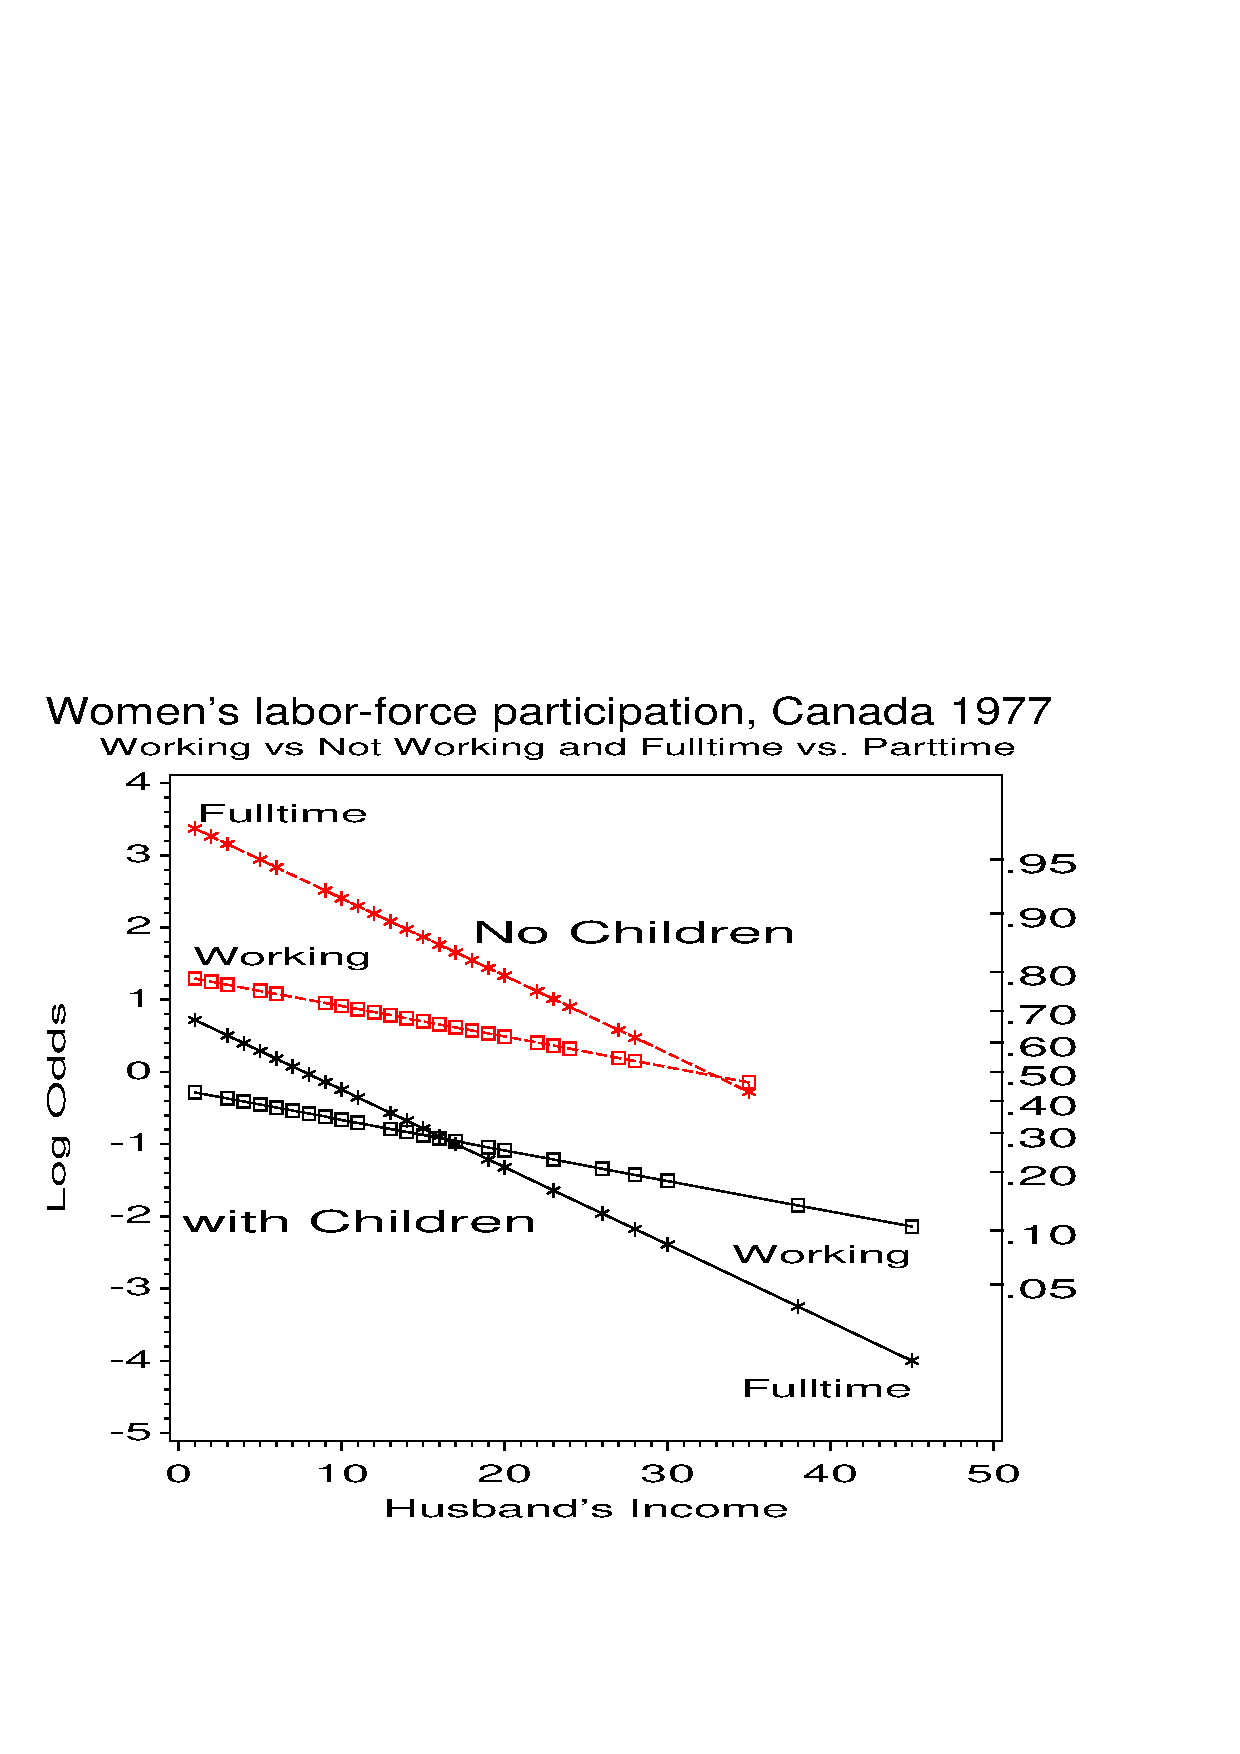
\includegraphics[scale=.7]{ch\thechapter/fig/wlfpart}
  \caption{Predicted log odds of working vs.\ not working, and of fulltime work vs.\ parttime work}\label{fig:wlfpart}
\end{figure}

To construct this graph, first join the separate results \Dsets\
into one.

\begin{listing}
*-- Merge the results to create one plot;
data both;
   set resultw(in=inw)
       resultf(in=inf);
   if inw then do;
      if children=1 then event='Working, with Children ';
      else event='Working, no Children ';
   end;
   else do;
      if children=1 then event='Fulltime, with Children ';
      else event='Fulltime, no Children ';
  end;
\end{listing}

Then, we can plot the log odds (or predicted probability) against
husband's income, using \pname{event} as to determine the curves to be
joined and labeled.
(The probability scale is constructed with the \macro{PSCALE}, and the
labels with an \ADS.  These steps are not similar to those described
in \exref{ex:arthrit10} and are
shown here).

\begin{listing}
proc gplot data=both;
   plot logit * husinc = event /
        anno=lbl nolegend frame vaxis=axis1;
   axis1 label=(a=90 'Log Odds') order=(-5 to 4);
   title2 'Working vs Not Working and Fulltime vs. Parttime';
   symbol1 v=dot    h=1.5 i=join l=3 c=red;
   symbol2 v=dot    h=1.5 i=join l=1 c=black;
   symbol3 v=circle h=1.5 i=join l=3 c=red;
   symbol4 v=circle h=1.5 i=join l=1 c=black;
\end{listing}
\end{Example}
